\resizebox{\textwidth}{!}{%
    \centering
    \scriptsize
    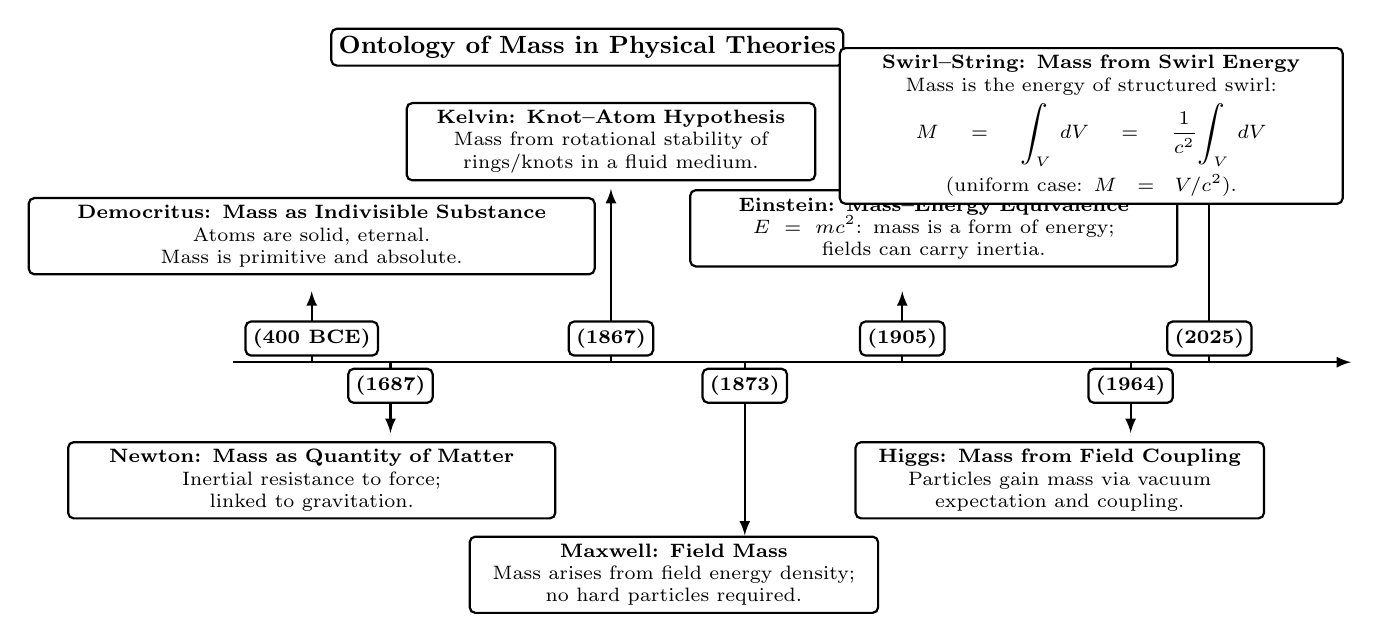
\begin{tikzpicture}[node distance=3.5cm, every node/.style={font=\scriptsize}, >=latex]
        \scriptsize

        % Timeline base
        \draw[->, thick] (-1,0) -- (13.2,0);

        % Arrows above timeline (short)
        \draw[->, thick] (0,0) -- (0,0.9);       % Pre-Socratics
        \draw[->, thick] (3.8,0) -- (3.8,2.2);   % Kelvin era
        \draw[->, thick] (7.5,0) -- (7.5,0.9);   % Einstein
        \draw[->, thick] (11.4,0) -- (11.4,2.2); % Swirl–String

        % Arrows below timeline (short)
        \draw[->, thick] (1.0,0) -- (1.0,-0.9);     % Newton
        \draw[->, thick] (5.5,0) -- (5.5,-2.2);     % Maxwell
        \draw[->, thick] (10.4,0) -- (10.4,-0.9);   % Higgs/modern

        % Root title cards (above)
        \node[draw, thick, rounded corners=2pt, fill=white, align=center, font=\bfseries ] at (0, .3)   {(400 BCE)};
        \node[draw, thick, rounded corners=2pt, fill=white, align=center, font=\bfseries ] at (3.8, .3) {(1867)};
        \node[draw, thick, rounded corners=2pt, fill=white, align=center, font=\bfseries ] at (7.5, .3) {(1905)};
        \node[draw, thick, rounded corners=2pt, fill=white, align=center, font=\bfseries ] at (11.4, .3){(2025)};

        % Root title cards (below)
        \node[draw, thick, rounded corners=2pt, fill=white, align=center, font=\bfseries ] at (1.0,- .3) {(1687)};
        \node[draw, thick, rounded corners=2pt, fill=white, align=center, font=\bfseries ] at (5.5,- .3) {(1873)};
        \node[draw, thick, rounded corners=2pt, fill=white, align=center, font=\bfseries ] at (10.4,- .3) {(1964)};

        % Label
        \node[draw, thick, fill=white, rounded corners=2pt, font=\small] at (3.5,4.0) {\textbf{Ontology of Mass in Physical Theories}};

        % Democritus (top-left)
        \node[draw, rounded corners=2pt, thick, align=center, fill=white, text width=7cm] at (0,1.6) {
            \textbf{Democritus: Mass as Indivisible Substance}\\
            Atoms are solid, eternal.\\
            Mass is primitive and absolute.
        };

        % Newton (below-left)
        \node[draw, rounded corners=2pt, thick, align=center, fill=white, text width=6cm] at (0,-1.5) {
            \textbf{Newton: Mass as Quantity of Matter}\\
            Inertial resistance to force;\\
            linked to gravitation.
        };

        % Kelvin (historical, top-mid)
        \node[draw, rounded corners=2pt, thick, align=center, fill=white, text width=5cm] at (3.8,2.8) {
            \textbf{Kelvin: Knot--Atom Hypothesis}\\
            Mass from rotational stability of\\
            rings/knots in a fluid medium.
        };

        % Maxwell (below-mid)
        \node[draw, rounded corners=2pt, thick, align=center, fill=white, text width=5cm] at (4.6,-2.7) {
            \textbf{Maxwell: Field Mass}\\
            Mass arises from field energy density;\\
            no hard particles required.
        };

        % Einstein (top-right-mid)
        \node[draw, rounded corners=2pt, thick, align=center, fill=white, text width=6cm] at (7.9,1.7) {
            \textbf{Einstein: Mass--Energy Equivalence}\\
            \(E=mc^2\): mass is a form of energy;\\
            fields can carry inertia.
        };

        % Higgs (bottom-right-mid)
        \node[draw, rounded corners=2pt, thick, align=center, fill=white, text width=5cm] at (9.5,-1.5) {
            \textbf{Higgs: Mass from Field Coupling}\\
            Particles gain mass via vacuum\\
            expectation and coupling.
        };

        % Swirl–String (top-right)
        \node[draw, rounded corners=2pt, thick, align=center, fill=white, text width=6.2cm] at (9.9,3.0) {
            \textbf{Swirl--String: Mass from Swirl Energy}\\
            Mass is the energy of structured swirl:\\[2pt]
            \( M \;=\; \displaystyle \int_{V}\rhoM\,dV \;=\; \frac{1}{c^{2}}\!\int_{V}\rhoE\,dV \)\\[2pt]
            (uniform case: \(M=\rhoE V / c^{2}\)).
        };

    \end{tikzpicture}
    \caption{\textbf{Evolution of the concept of mass:} from atomistic substance (Democritus), through Newtonian inertia and field--theoretic mass (Maxwell, Higgs), to a swirl--string fluid--topological model where mass equals swirl energy divided by \(c^{2}\). Historical labels are retained for context; modern terminology avoids mechanical ether phrasing.}\label{fig:OntologyOfMass}
}